% Artyom Voronin
%  __  __           _      _ 
% |  \/  | ___   __| | ___| |
% | |\/| |/ _ \ / _` |/ _ \ |
% | |  | | (_) | (_| |  __/ |
% |_|  |_|\___/ \__,_|\___|_|
%                            
% Brno, 2020

% -------------------------------------------------------
% Section
% -------------------------------------------------------
\chapter{First Principle Modeling}
First-principle modeling is a common engineering modeling approach. Models
developed using physical laws such as energy and mass balance, heat
transfer, and so on. First-principle modeling requires knowledge of the
system and the physical processes that take place in this system.

First principle models (FPMs) are usually designed in the form of a system
of differential equations, algebraic differential equations, transfer
functions, state-space systems, etc.  In designing FPMs, it is necessary to
determine the assumptions and simplifications that correspond to the level
of technical resolution in a particular problem.

This chapter introduces the design of a double-acting pneumatic piston
assembly model, including sensors using a first-principle modeling
approach. 

% TODO Isermann Fault Detection str 72
%Measurements, Identification.

% Nonlinear dynamic modeling  Isermann FDS str. 84

% -------------------------------------------------------
%  __ _  ___ _ __   ___ _ __ __ _| |
% / _` |/ _ \ '_ \ / _ \ '__/ _` | |
%| (_| |  __/ | | |  __/ | | (_| | |
% \__, |\___|_| |_|\___|_|  \__,_|_|
% |___/                             
% -------------------------------------------------------
\section{General physical principles}
\paragraph{Assumptions}\label{assumptions}

\begin{enumerate}
    \item The effect of accelerated air mass is neglected. 
    \item The gas is ideal. 
    \item All the thermal processes are adiabatic.
\end{enumerate}

\paragraph{Simplifications}
Throttle modeling and adjustment dampers require measurements that were
unfortunately not available. In the case of throttle valves, the parameters
of the throttle valves were combined with the parameters of the control
solenoid valve.


\paragraph{Equation of state}
Equation of state for an ideal gas \ref{eq:equation_of_state}, describe the relationships between
temperature, mass, pressure and volume of the gas, where $R=287.1 \rm [Jkg^{-1}K^{-1}]$ is an ideal gas
constant.

\begin{align}
    pV = mRT
    \label{eq:equation_of_state}
\end{align} 

\paragraph{Adiabatic process}
All processes take place without heat exchange with the environment by
given equation \ref{eq:adiabatic_process}, where $\kappa = c_p/c_v$ is a
heat capacity ratio.

\begin{align}
     p_1V_1^{\kappa} =  p_2V_2^{\kappa} = const
    \label{eq:adiabatic_process}
\end{align}

Relation between heat capacities and an ideal gas constant is given
by Mayer's equation as $c_p = c_v + R$.



\paragraph{Bernouilli's principle}
Bernouilli's equation \ref{eq:bernoullis_principle} describes flow
dynamics as a sum of kinetic, potential and internal energies.

\begin{align}
    H_1 + \frac{mw_1^2}{2} + mgz_1 + Q = H_2 + \frac{mw_2^2}{2} + mgz_w +
    W_T
    \label{eq:bernoullis_principle}
\end{align}

Transition to specific values:
\begin{align}
    h_1- h_2 = -\int_1^2 v dp = c_p(T_1-T_2) = 
    c_p T_1\left(1-\frac{T_2}{T_1}\right)
    \label{eq:etalpi_sub}
\end{align}

\paragraph{Continuity equation}
Continuity equation \ref{eq:continuity_equation} describes a mass flow
through a control volume.

\begin{align}
    \dot{m} = S_1 w_1 \rho_1 = S_2 w_2 \rho_2 = const
    \label{eq:continuity_equation}
\end{align}

\section{Air Expansion}\label{sec:air_expansion}
Air expansion from the reservoir, one of the fundamental sets of equations
used in pneumatic elements. 

\begin{figure}[h!]
    \centering
    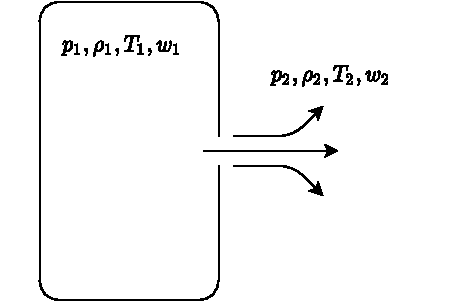
\includegraphics[width=0.5\textwidth]{air_tank.pdf}
    \caption{Air expansion from tank}
    \label{fig:air_expansion}
\end{figure}

Assuming that $W_T = 0, Q = 0$ there is no work and heat shared with the
the environment, there is no difference in height $z_1 = z_2$ and
the velocity difference is vast $w_2 << w_1$, applying equation
\ref{eq:bernoullis_principle}, get \ref{eq:w2}.


\begin{align}
    w_2 = \sqrt{2(h_1 - h_2)}
    \label{eq:w2}
\end{align}

\begin{align}
    w_2 = \sqrt{2c_p T_1 \left(1-\frac{T_2}{T_1}\right)}
    \label{eq:w2}
\end{align}

where 

\begin{align}
    T_1 = \frac{p_1}{R \rho_1} && 
    c_p = R  \left( \frac{\kappa}{\kappa-1} \right)   &&
    \frac{T_2}{T_1} = \left(\frac{p_2}{p_1} \right)^{\frac{\kappa - 1}{\kappa}}
    \label{eq:helpers}
\end{align}

Combine equations \ref{eq:w2}, \ref{eq:helpers} to get air expansion
velocity \ref{eq:w2_final}.

\begin{align}
    w_2 =
    \sqrt{2 \frac{\kappa}{\kappa-1} \frac{p_1}{\rho_1} 
    \left[(1-\left(\frac{p_2}{p_1}\right)^\frac{\kappa-1}{\kappa}\right]}
    \label{eq:w2_final}
\end{align}

From equations \ref{eq:helpers} express air density \ref{eq:rho2}.
\begin{align}
    \rho_2 = \frac{p_1}{RT_1} \left(\frac{p_2}{p_1}\right)^{\frac{1}{\kappa}}
    \label{eq:rho2}
\end{align}

Using continuity equation \ref{eq:continuity_equation} and
\ref{eq:w2_final} describe mass flow as \ref{eq:dot_m}:

\begin{align}
    \dot{m} = A p_1 \sqrt{\frac{2}{RT_1}}
    \sqrt{\frac{\kappa}{\kappa-1} \frac{p_1}{\rho_1} 
    \left[(1-\left(\frac{p_2}{p_1}\right)^\frac{\kappa-1}{\kappa}\right]}
    \label{eq:dot_m}
\end{align}

where \ref{eq:psi} is the outflow function.

\begin{align}
    \psi\left(\frac{p_2}{p_1}\right) =  
    \sqrt{\frac{\kappa}{\kappa-1} \frac{p_1}{\rho_1} 
    \left[(1-\left(\frac{p_2}{p_1}\right)^\frac{\kappa-1}{\kappa}\right]}
    \label{eq:psi}
\end{align}

Finally mass flow expansion from the reservoir is given by equation
\ref{eq:mass_flow}:
\begin{align}
    \dot{m} = A p_1\sqrt{\frac{2}{RT_1}} \cdot \psi\left(\frac{p_2}{p_1}\right)
    \label{eq:mass_flow}
\end{align}


\paragraph{Critical flow velocity}
The outflow function depends on the pressure ratio $p_2/p_1$. This function
has a maximum value when the critical pressure is reached; the mass flow
becomes chocked. Critical pressure is presented by \ref{eq:beta_k}. For the
overcritical pressure ratio, the mass flow depends only on $p_1$ and $T_1$
\cite{isermann}.

\begin{align}
    &\left(\frac{p_2}{p_1}\right)_{crit} =
    \left(\frac{2}{\kappa+1}\right)^\frac{\kappa}{\kappa-1}=\beta_k
    \label{eq:beta_k}
\end{align}

Critical pressure for air is $\beta_k = 0.528$ and critical velocity is
give by outflow function \ref{eq:psi_max}. Combine equations for
overcritical and undercritical pressure ratio using equations
\ref{eq:beta_k}, \ref{eq:psi_max} we get the final equation for outflow
function \ref{eq:psi_final}.

\begin{align}
    &\psi_{max} (\beta_k) = 
    \left(\frac{2}{\kappa+1}\right)^\frac{\kappa}{\kappa-1}\sqrt{\frac{\kappa}{\kappa+1}}
    = 0.484
    \label{eq:psi_max}
\end{align}

\begin{align}
\psi\left(\frac{p_2}{p_1}\right) = 
    \begin{cases}
    \sqrt{\frac{\kappa}{\kappa-1} \frac{p_1}{\rho_1} 
    \left[(1-\left(\frac{p_2}{p_1}\right)^\frac{\kappa-1}{\kappa}\right]}
    & 0.528 <\frac{p_2}{p_1} \le 1 \\
    \left(\frac{2}{\kappa +1}\right)^{\frac{1}{\kappa+1}}
    \sqrt{\frac{\kappa}{\kappa +1}} & 0 \le \frac{p2}{p1} \le 0.528\\
    \end{cases}
\label{eq:psi_final}
\end{align}

A detailed derivation of the equation \ref{eq:psi_final} can be found in
\cite{isermann},\cite{}.


%\begin{tabular}{ |c|c|c| }
%    \hline
%    $p$                     & $Pa$              & pressure \\
%    $V$                     & $m^3$             & volume \\
%    $m$                     & $kg$              & mass \\
%    $n$                     & $mol$             & amount of substance \\
%    $R$                     & $Jkg^{-1}K^{-1}$  & ideal gas constant \\
%    $r$                     & $Jkg^{-1}K^{-1}$  & mass-specific gas constant \\
%    $T$                     & $K$               & temperature \\
%    $S$                     & $m$               & area \\
%    $z$                     & $m$               & height \\
%    $w$                     & $ms^{-1}$         & flow speed \\
%    $H$                     & $J$               & enthalpy \\
%    $\nu$                   & $m^3kg^{-1}$      & specific volume \\
%    $Q$                     & $J$               & heat shared with
%                                                    environment \\
%    $W_T$                   & $J$               & work \\
%    $c_p$                   & $Jkg^{-1}K^{-1}$  & is the specific heat
%                                                    at constant pressure \\
%    $c_v$                   & $Jkg^{-1}K^{-1}$  & is the specific heat at constant volume\\
%    $g=9.81$                & $ms^{-2}$         & gravity acceleration \\
%    $\kappa=1.4\text{(air)}$& $-$               & heat capacity ratio
%                                                    (isentropic expansion factor)\\
%    \hline
%\end{tabular}


%\begin{tabular}{ |c|c|c| }
%    \hline
%    $\dot{m}$                   & $kgs^{-1}$  & mass flow \\
%    $c$                         & $ms^{-2}$   & speed of sound \\
%    $w_k$                       & $ms^{-2}$   & critical flow velocity \\
%    $\psi$                      & $-$         & flow coefficient \\
%    $\psi_{max}$                & $-$         & critical flow coefficient \\
%    $\beta$                     & $-$         & ration of pressure
%                                                    differential \\
%    $\beta_k$                   & $-$         & critical ratio of pressure
%                                                    differential \\
%
%    \hline
%\end{tabular}

% -------------------------------------------------------
% _ __  _ __ ___  ___ ___ _   _ _ __ ___ 
%| '_ \| '__/ _ \/ __/ __| | | | '__/ _ \
%| |_) | | |  __/\__ \__ \ |_| | | |  __/
%| .__/|_|  \___||___/___/\__,_|_|  \___|
%|_|                                     
% -------------------------------------------------------
\section{Pneumatic Piston Pressure Model}

%\begin{tabular}{ |c|c|c| }
%    \hline
%    $p_A, p_B$              & $Pa$              & pressure in chamber A, B \\
%    $\dot{m_A}, \dot{m_B}$  & $kg \cdot s^{-1}$ & mass flow on way to chamber A, B \\
%    $S_A, S_B$              & $m^2$             & piston area  \\
%    $V_A, V_B$              & $m^3$             & volume of chamber A,B \\
%    $V_{0A}, V_{0B}$        & $m^3$             & "dead" volume of chamber A,B \\
%    $m$                     & $kg$              & piston mass\\
%    $F_{load}$              & $N$               & load \\
%    $x$                     & $m$               & piston position \\
%    $l$                     & $m$               & maximum piston position \\
%    \hline
%\end{tabular}
A construction principle of the double-acting pneumatic piston is shown in
the figure \ref{fig:pist_chamb}.  There are two chambers connected to the control valve.
If the control valve is connected to chamber A, the supply pressure drives
mass flow into chamber A. At the same time, the port at chamber B is
connected to the ambient. Due to the pressure difference between chambers,
pneumatic piston stroke start moving in a positive direction. 
After the bound is reached and the pressure in the chamber equalizes to
supply pressure, there is no longer any mass flow coming inside.


\begin{figure}[h!]
    \centering
    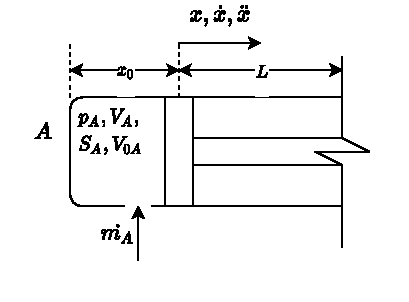
\includegraphics[width=0.6\textwidth]{pressure_chamber.pdf}
    \caption{Piston chamber}
    \label{fig:pist_chamb}
\end{figure}

Assuming an isothermal process, derivation of the equation of state $m =
\rho V$ get the equation \ref{eq:dm_state}. 

\begin{align}
    \dot{m} = \dot{\rho} V + \rho \dot{V}
    \label{eq:dm_state}
\end{align}

where

\begin{align}
    \rho = \frac{p}{RT} &&
    \dot{\rho} = \frac{\dot{p}}{RT} 
\end{align}

Equation \ref{eq:pressure1} describe pressure difference in chamber due
mass flow.
\begin{align}
    \dot{p} = - \frac{p}{V}\dot{V} + \frac{RT}{V}\dot{m}
    \label{eq:pressure1}
\end{align}


For the adiabatic model of the pressure difference in the chamber,
moreover, heat capacity ratio added
\ref{eq:pressure_adiabatic_simple_model}.

\begin{align}
    \dot{p} = - \frac{\kappa p}{V}\dot{V} + \frac{\kappa RT}{V}\dot{m}
    \label{eq:pressure_adiabatic_simple_model}
\end{align}
Volumes of the chambers can be represented concerning figure
\ref{fig:pist_chamb} as volumes equations \ref{eq:volumes}.

\begin{align}
    V_A = S_A x + V_{0A} \\
    V_B = S_B (L-x) + V_{0B} \\
    \dot{V}_A = S_A \dot{x} \\
    \dot{V}_B = - S_B \dot{x}
    \label{eq:volumes}
\end{align}

The pneumatic piston with chambers A, B is described by the system of
differential equations \ref{eq:p_A}, \ref{eq:p_B}. These equations describe a pneumatic
cylinder entirely. Furthermore, all the parameters can be directly measured
or found in the datasheet \cite{}.

\begin{align}
    \dot{p_A} = \frac{\kappa}{S_A x + V_{0A}} \left(- p_A S_A\dot{x} +
    RT_A\dot{m_A} \right)
    \label{eq:p_A}
\end{align}

\begin{align}
    \dot{p_B} = \frac{\kappa}{S_B (L-x) + V_{0B}} \left(p_B S_B\dot{x} +
    RT_B\dot{m_B} \right)
    \label{eq:p_B}
\end{align}


\section{Control Valve Model}
The pneumatic control valve manipulates air mass flow to connect piston
chambers with supply and ambient pressure lines. There are different
approaches to model pneumatic control valve describes \cite{}, \cite{}.
Demonstration device includes 5/2 bistable solenoid valve
\ref{fig:device_scheme}. The movable part, valve spool driven by a magnetic
field, can be in the two positions, where one of the chambers connects to
the supply pressure line, another to ambient. A digital input signal
switches between these two positions \ref{}.  Equation \ref{eq:input_u},
describe the input signal $u \in \langle-1,1\rangle$, which regulates the
spool movement to acquire one of
the states. 

\begin{align}
    u =
    \begin{cases}
        -1 & \text{discharge the chamber} \\
       \  1  & \text{filling the chamber} 
    \end{cases}
    \label{eq:input_u}
\end{align} 

Spool dynamic and pressure lines transport delay can be modeled as a 1dof
system with the time constant $T$ and delay $\tau$ \ref{eq:spool_dynamic}. For
more precise control and modeling of the valve system, valve dead zones can
be considered \ref{eq:deadzone}.

\begin{equation}
    G(s) = \frac{1}{T s + 1}e^{-\tau s}
    \label{eq:spool_dynamic}
\end{equation}


\begin{equation}
    u_z = 
    \begin{cases}
        g_z(u) < 0 &, \text{ if } u \le u_n \\
        0          &, \text{ if } u_n < u < u_p \\
        h_z(u) > 0 &, \text{ if } u \ge u_p \\
    \end{cases}  
    \label{eq:deadzone}
\end{equation}



To parametrize the pneumatic valve discharge coefficient (coefficient of
contraction) can be used. This parameter must be determined experimentally.
The discharge coefficient \ref{eq:coefficient_of_contraction} is the ratio
between the equivalent area of the opened flow path and the maximum area of
this path. The equivalent area limits the maximum mass flow value. 

\begin{align}
    C_d = \frac{S_{eq}}{S_{max}}
    \label{eq:coefficient_of_contraction}
\end{align}

With respect to outflow function \ref{eq:psi_final} and mass flow function
\ref{eq:mass_flow} derived in section \ref{sec:air_expansion},  control
valve equation is given \ref{eq:flow}.

\begin{align}
    \dot{m} = u S_{max} C_d p_1 \sqrt{\frac{2}{RT_1}}
    \cdot \psi\left(\frac{p_2}{p_1}\right)
    \label{eq:flow}
\end{align}



Using the notation introduced on the schemes \ref{fig:device_scheme},
\ref{fig:pist_chamb} we compile a complete set of equations for the
description of the behavior of a
pneumatic solenoid valve \ref{eq:m_A_final}, \ref{eq:m_B_final}.

\textbf{For filling the chamber:}
\begin{itemize}
\item $p_1 = p_s$ 
\item $p_2 = p_A \text{ or } p_B$
\item $T_1 = T_s$
\end{itemize}

\textbf{For discharge the chamber:}
\begin{itemize}
\item $p_1 = p_A \text{ or } p_B$
\item $p_2 = p_0$
\item $T_1 = T_A, T_B$
\end{itemize}

where $p_s$ is supply pressure. $p_0$ atmospheric pressure, $T_A = T_B =
T_0$ ambient temperature.

\begin{align}
    \dot{m}_A =
    \begin{cases}
        u S_v C_d p_s \sqrt{\frac{2}{RT_s}}
        \cdot \psi\left(\frac{p_A}{p_s}\right)  &,   u \in (0, 1 \rangle \\
        u S_v C_d p_A \sqrt{\frac{2}{RT_A}}
        \cdot \psi\left(\frac{p_0}{p_A}\right)  &,   u \in \langle -1, 0) \\
    \end{cases}
    \label{eq:m_A_final}
\end{align}

\begin{align}
    \dot{m}_B =
    \begin{cases}
        u S_v C_d p_s \sqrt{\frac{2}{RT_s}}
        \cdot \psi\left(\frac{p_B}{p_s}\right)  &,   u \in (0, 1 \rangle \\
        u S_v C_d p_A \sqrt{\frac{2}{RT_B}}
        \cdot \psi\left(\frac{p_0}{p_B}\right)  &,   u \in \langle -1, 0) \\
    \end{cases}
    \label{eq:m_B_final}
\end{align}

% TODO
%\subsection{Valve model} 
%\begin{tabular}{ |c|c|c| }
%    \hline
%    $S_{eq}$                & $m^2$         & Equivalent cross section \\
%    $S_{max}$               & $m^2$         & Maximum cross section \\
%    $Cd$                    & $-$           & Coefficient of contraction \\
%    $u$                     & $-$           & Regulation variable \\
%    \hline
%\end{tabular}


% -------------------------------------------------------
% _ __ ___   ___  ___| |__   __ _ _ __ (_) ___ 
%| '_ ` _ \ / _ \/ __| '_ \ / _` | '_ \| |/ __|
%| | | | | |  __/ (__| | | | (_| | | | | | (__ 
%|_| |_| |_|\___|\___|_| |_|\__,_|_| |_|_|\___|
% -------------------------------------------------------
\section{Mechanical assembly}
\subsection{Equation of motion}

The motion of the pneumatic piston mechanism describes in terms of the
general 1dof dynamical equation \ref{eq:1dof}. 

\begin{equation}
    m\ddot{x} + b\dot{x} + kx = u
    \label{eq:1dof}
\end{equation}

In the case of the pneumatic piston, equation \ref{eq:1dof}
transforms into and equation \ref{eq:mechanical}.

\begin{equation}
    (M + M_L) \ddot{x} + F_{d} + F_g + F_{hs} + F_f  = F_p
    \label{eq:mechanical}
\end{equation}

Where $M$ represents a mass of the all moveable part of the piston,
$M_L$ is load mass, $F_g$ gravity force acting to mechanical moving assembly,
$F_{hs}$ - models endpoints (hard stop),
$F_{d}$ represents dampers (shock absorbers) acted at endpoints,
$F_f$ describe Coulomb and viscous friction,
$F_{p}$ is a force produced by the pneumatic piston and given by equation \ref{eq:pneum}.

\begin{equation}
    F_p = P_A S_A - P_B S_B - P_0 S_0
    \label{eq:pneum}
\end{equation}

\paragraph{Friction} Friction force was modeled as a Coulomb and viscous
friction\ref{eq:friction_force}.

\begin{equation}
    F_f = F_C \cdot \text{sign}(\dot{x}) + B_v \dot{x}
    \label{eq:friction_force}
\end{equation}


\subsection{Hard stop}
The endpoint's material resistance can be represented as springs and
dampers acting as one-way bound \ref{eq:hard_stop}
The parameters $K$, $D$  have a significant impact on the numerical stability
of the simulation system; therefore, they were tuned concerning stable
performances.

\begin{align}
    F_{hs} =
    \begin{cases}
        K_p(x-g_p) + D_pv & \text{for } x \ge g_p \\
        0 & \text{for } g_n < x < g_p \\
        K_n(x-g_n) + D_nv & \text{for } x \le g_n \\
    \end{cases}
    \label{eq:hard_stop}
\end{align}


\subsection{Endpoint dampers}
There are two types of dampers installed in demonstration device. One pair
is adjustable, and other stable.  Endpoint dampers were modeled in the same
way as a hard stop \label{eq:hard_stop}, emphasizing damping coefficient
$D$. 

% -------------------------------------------------------
% ___  ___ _ __  ___  ___  _ __ ___ 
%/ __|/ _ \ '_ \/ __|/ _ \| '__/ __|
%\__ \  __/ | | \__ \ (_) | |  \__ \
%|___/\___|_| |_|___/\___/|_|  |___/
% -------------------------------------------------------
\section{Sensors Modeling}
\begin{figure}[h!]
    \centering
    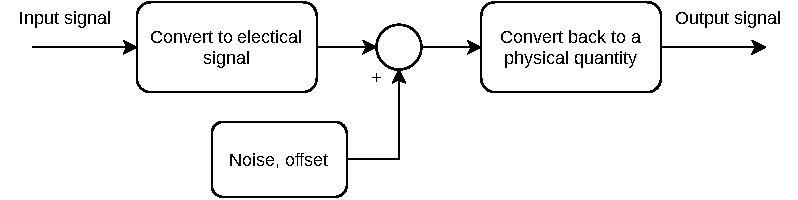
\includegraphics[width=0.6\textwidth]{fpm_signals_modeling.pdf}
    \caption{Sensors Modeling Diagram}
    \label{fig:sig_mod_diag}
\end{figure}


Modeling sensors include converting the measured physical signals to an
analog or digital signal, adding noise and offset parameters to have an
option to model faults conditions, and after converting back to the
sensor's measured units \ref{fig:sig_mod_diag}. 

\paragraph{Flow sensors}
Flow sensors are a typical representative of a comfortable sensor to
implement by converting the units used in the model $\rm [kg/s]$ into a voltage
$\rm [V]$ concerning the datasheet. Then added measurement noise and the
possibility to add offset for further experiments and finally, converting
back to physical quantity with respect to the sensor measuring in $\rm
[l/min]$.

\paragraph{Strain Gauge}
Strain Gauge was modeled similarly as a flow sensor with the possibility of
experimentation with the magnitude of noise and offset.

\paragraph{Accelerometer}
The accelerometer attached to the moving part of the system was modeled
using a transfer function concerning the datasheet and estimated magnitude
of the measurement noise. It's also the ability to add optionally offset or
off the sensor itself.

\paragraph{Proximity sensors} In the case of digital signals such as
proximity sensors, it is sufficient to control the boundaries at which the
sensor is switched on.


\paragraph{Encoder}
The demonstration device includes a very precise linear magnetic encoder
with a resolution $\approx 7 \rm \mu m$. This sensor provides an almost
clean signal that gives an option to extract velocity signal by numerical
derivation.  However, to model this type of encoder with parameters of real
encoder requires a minimum sample time in the range of $\rm \mu s$. Due to
this fact model of the encoder was embedded, but the output is taken
directly from the model.

\paragraph{Not implemented}

Sensors that are difficult to implement or have not been included in the
model have not been implemented. These sensors include microphones, a
static accelerometer mounted on a construction pad, an air pressure sensor
because the air reservoir was not modeled in this work, temperature
sensors.

% -------------------------------------------------------
%(_) __| | ___ _ __ | |_ 
%| |/ _` |/ _ \ '_ \| __|
%| | (_| |  __/ | | | |_ 
%|_|\__,_|\___|_| |_|\__|
% -------------------------------------------------------
\section{Parameter Estimation}

To achieve closer behavior to the real system, it is necessary to determine
all the parameters of the model.  There are parameters given as physical
constants, or they can be directly measured or determined in the datasheet.
Parameters that do not fall under these kinds must be deducted from the
measurement.

According to the simplification estimation process, throttle valves and
solenoid valve parameters were combined into two valve coefficients
$C_{i,in}, C_{i,out}$ in both input and output directions \ref{eq:valve_estimation}.
\begin{align}
    \dot{m}_{i,in} = u(t)\cdot \boldsymbol{C_{i,in}} p_1 \sqrt{\frac{2}{RT_1}}
    \cdot \psi\left(\frac{p_2}{p_1}\right) &&
    \dot{m}_{i,out} = u(t)\cdot \boldsymbol{C_{i,out}} p_1 \sqrt{\frac{2}{RT_1}}
    \cdot \psi\left(\frac{p_2}{p_1}\right)
    \label{eq:valve_estimation}
\end{align}

where $i$ are ports to chambers $A, B$.


Solenoid valve spool dynamic was estimated with respect to equation
\ref{eq:spool_dynamic}
in different displacement measurements. 

Pneumatic piston parameters were taken from the datasheet, and the remaining
such as dead volumes $V_{0A}$ and $V_{0B}$ estimated approximately.

Hard stop endpoints were determined from the construction design of a
particular pneumatic piston. The values of the damping and spring were
estimated to perform their functions and at the same time maintain
numerical stability.

Adjustment dampers were estimated from displacement measurement as $b_b$,
$b_u$ parameters. The bounding range was directly measured from the
displacement measurements.

\begin{table}[h]
    \centering
    \begin{tabular}{|c|c|}
        \hline
        \textbf{parameter} & \textbf{description}  \\
        \hline
        $C_{A,in}$      & valve coefficient connected to input path to  A chamber \\
        $C_{A,output}$  & valve coefficient connected to output path from A chamber \\
        $C_{B,in}$      & valve coefficient connected to input path to  B chamber \\
        $C_{B,output}$  & valve coefficient connected to output path from B chamber \\
        $b_{up}$        & upper damper value  \\
        $b_{bot}$       & bottom damper value \\
        \hline
    \end{tabular}
    \caption{Parameters to reestimate for different fault conditions}
    \label{tab:est_params}
\end{table}

\section{Model performance}

\begin{figure}[h!]
    \centering
    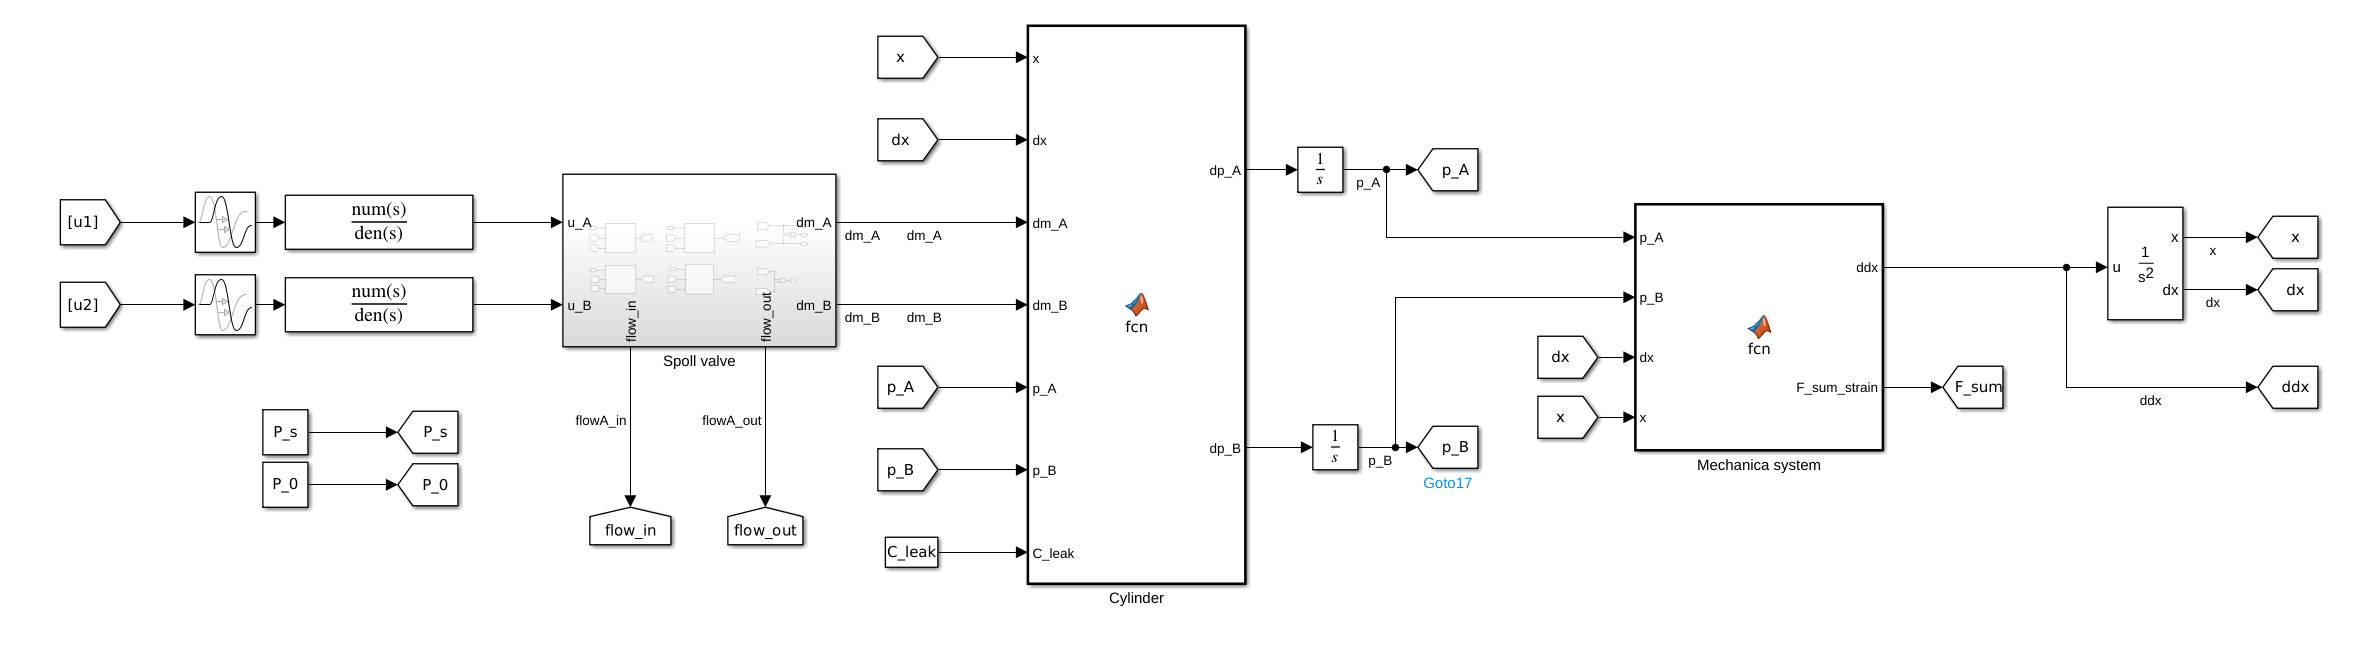
\includegraphics[width=1\textwidth]{fpm_model.png}
    \caption{First Principle model implementation in Simulink}
    \label{fig:fpm_simulink}
\end{figure}

The model was implemented using the Matlab/Simulink software using basic
Simulink operations and the Matlab-Function block. The model shows good
numerical stability and allows to perform simulations with a fix step
solver with a sampling time of $1\cdot 10^{-3} \rm\ s$. Which significantly speeds up the
simulations and the process of parameter estimation. Figure
\ref{fig:fpm_simulink} shows
the central part of the model in the Simulink environment.


The resulting behavior of the system after parameter estimation on health
conditions data is shown in Figure \ref{fig:fpm_perfomance}. However, it is
possible to reestimate the basic parameters \ref{tab:est_params} and thus
realize the behavior of the system closer to the fault state.

\begin{figure}[!ht]
    \centering
    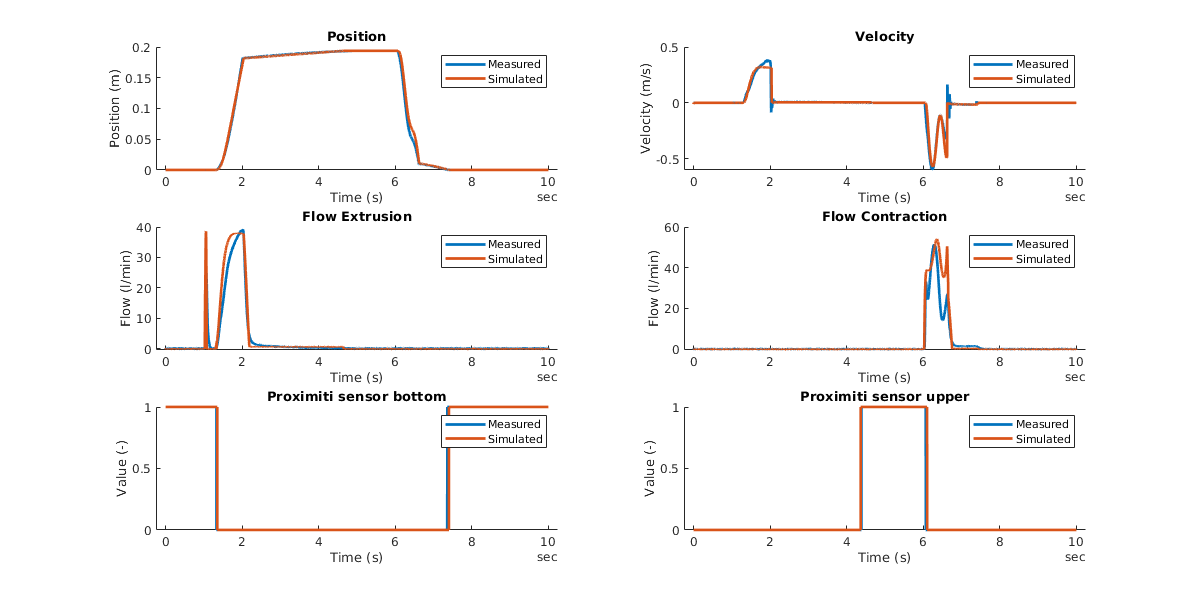
\includegraphics[width=1\textwidth]{fpm_perfomance.png}
    \caption{Comparison between measurement and model response}
    \label{fig:fpm_perfomance}
\end{figure}


Figure \ref{fig:fpm_fault_example} shows the simulation system
response with different estimated parameters for the fault states caused by
the Throttle valve 2. In the case of position, the measured and simulation
signals practically overlap.

\begin{figure}[!ht]
    \centering
    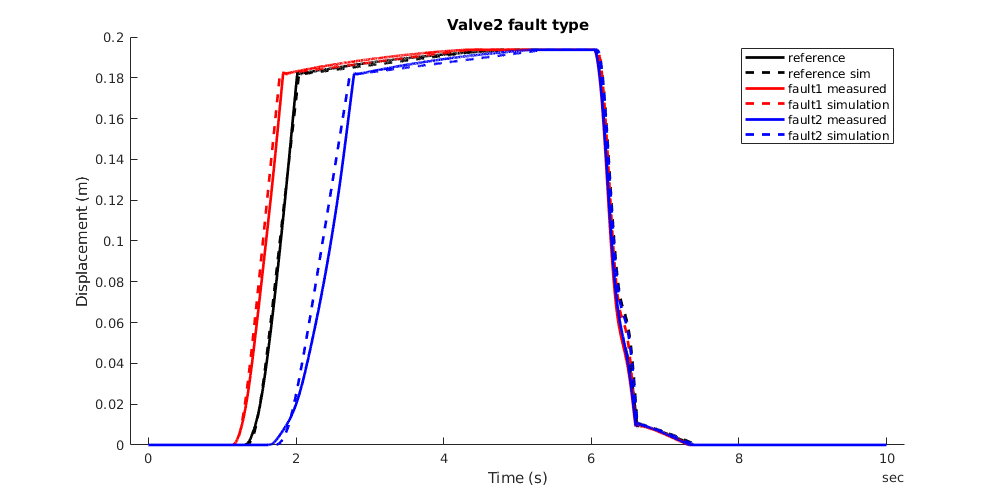
\includegraphics[width=1\textwidth]{fpm_fault_example.png}
    \caption{Simulation model performance in different fault conditions}
    \label{fig:fpm_fault_example}
\end{figure}

